
%(BEGIN_QUESTION)
% Copyright 2006, Tony R. Kuphaldt, released under the Creative Commons Attribution License (v 1.0)
% This means you may do almost anything with this work of mine, so long as you give me proper credit

Does the output pressure of this relay {\it increase} with increasing input pressure, or {\it decrease} with increasing input pressure?  In other words, is it a {\it direct-acting} or {\it reverse acting} type of relay?

$$\includegraphics[width=15.5cm]{i00197x01.eps}$$

\vskip 20pt \vbox{\hrule \hbox{\strut \vrule{} {\bf Suggestions for Socratic discussion} \vrule} \hrule}

\begin{itemize}
\item{} Explain this comparison: ``A relay is to a pilot what a transistor is to a hand switch''
\item{} How do you think a leak or tear in the diaphragm would affect the behavior of this relay?
\item{} How do you think a plugged orifice would affect the behavior of this relay?
\item{} How do you think variations in the supply pressure would affect the behavior of this relay?
\end{itemize}

\underbar{file i00197}
%(END_QUESTION)





%(BEGIN_ANSWER)


%(END_ANSWER)





%(BEGIN_NOTES)

The output pressure increases with increasing input pressure: it is a {\it direct-acting} relay.






\vfil \eject

\noindent
{\bf Summary Quiz:}

Identify a condition in this pneumatic relay that would cause the output pressure to decrease:

$$\includegraphics[width=15.5cm]{i00197x02.eps}$$

\begin{itemize}
\item{} The input pressure increases
\vskip 5pt 
\item{} Debris plugs the pilot valve
\vskip 5pt 
\item{} Debris plugs the vent hole
\vskip 5pt 
\item{} The supply pressure increases
\vskip 5pt 
\item{} Air temperature increases
\vskip 5pt 
\item{} Debris plugs the orifice
\vskip 5pt 
\item{} Air temperature decreases
\end{itemize}


%INDEX% Basics, pneumatics: relay action (direct vs. reverse)

%(END_NOTES)


